\chapter{Реализация и экспериментальная проверка Алгоритмов геолокации}

\section{Состав и структура реализованного программного обеспечения}

Нужно охарактеризовать реализованное ПО: является ли оно настольной программной для Windows, или веб-приложением в форме сайта/веб-сервиса, или модулем/подключаемой библиотекой, или \dots. Также нужно перечислить, из чего оно состоит: какие исполняемые файлы и их назначение, конфигурационные файлы, файлы баз данных, требования к программному и аппаратному окружению, и т.п.

Если реализованное приложение достаточно обширно, этот раздел может быть
разделен на несколько: один с общим описанием, и по одному на подсистемы самого
верхнего уровня.

\section{Описание обучающих и тестовых данных}

Для тестирования разработанной системы использовались снимки \texttt{Google Street View} из 10 городов снятые в панорамном режиме с разрешением $ 224\times224 $. Код, генерирующий эти снимки представлен на листинге \ref{lst:Gen}.

Так как \texttt{API Google Street View} отвечает картинкой и не для всех координат в городе существуют панорамы, отфильтровывать ошибки можно просто используя размер картинки
как хэш функцию. Коллизии маловероятны из-за того что обычно панорамы на порядок отличаются по размеру от картинки, обозначающей ошибку. Интересующая нас часть листинга представлена ниже.

\begin{lstlisting}[language=python, float=tb,frame=lines,label=lst:frag1]
# check if the downloaded image was invalid and if so remove it
...
if os.path.isfile(filepath):
	size = os.path.getsize(filepath)
	if size == FAILED_DOWNLOAD_IMAGE_SIZE:
		os.remove(filepath)
		misses += 1
	else:
		num_imgs += 1
...
\end{lstlisting}

Снимки генерируются методом случайного сдвига точки к которой делается запрос и случайного поворота.

Для разделения на тестовую и обучающую выборки также используются скрипты.

\section{Результаты экспериментов}

\subsection{Эксперимент с 1 изображением}

Было проведено обучение модели на основе свёрточной сети \texttt{resnet34} с использованием подхода \texttt{transfer learning}. Для оптимизации использовался 
метод Стохастического градиентного спуска с параметрами $ \mbox{размер шага} = 0,001 и \mbox{momentum} = 0.9$. В процессе обучения каждые 7 шагов раз

\texttt{F1}-взвешенная оценка для классификации $ 0.5101 $

\begin{figure}
	\centering
	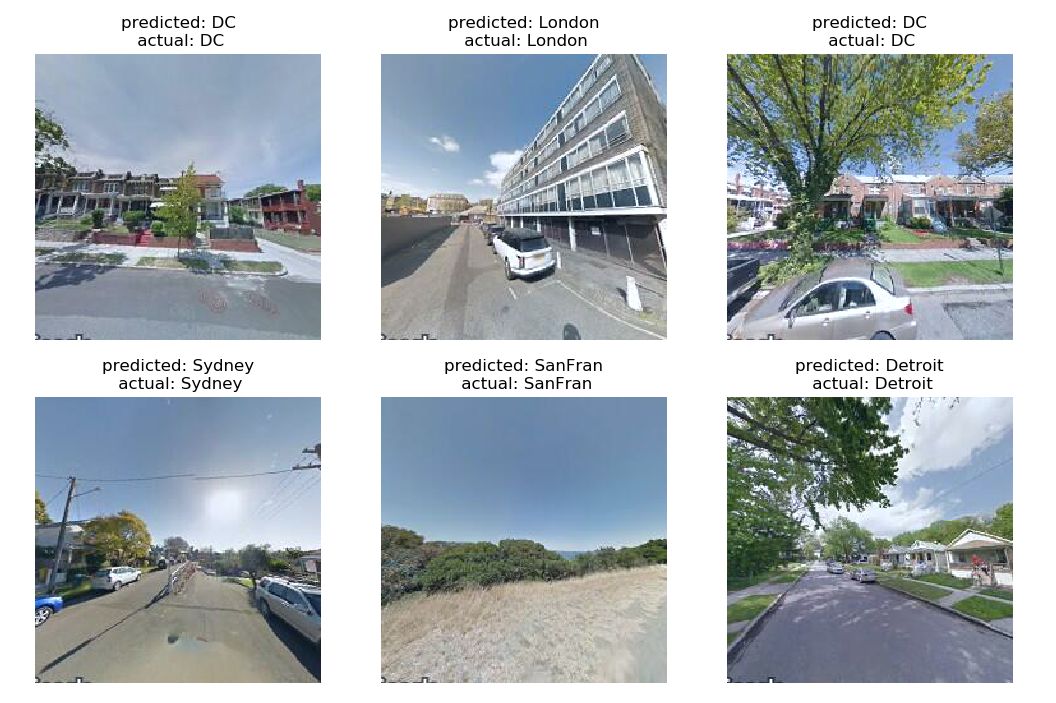
\includegraphics[width=0.9\linewidth]{img/res1im}
	\caption{Результат обучения модели с resNet18 по 1 изображению}
	\label{fig:res1im}
\end{figure}

\begin{figure}[h]
	\centering
	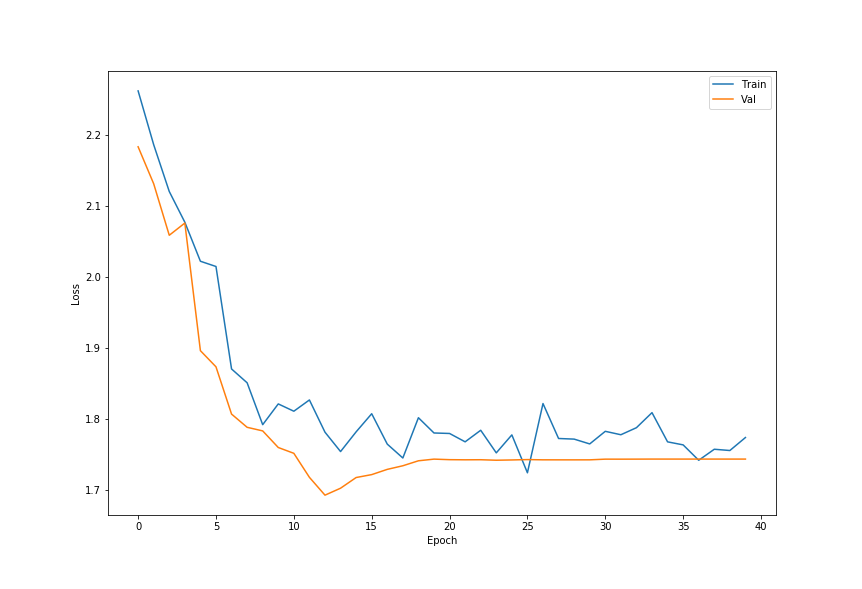
\includegraphics[width=0.8\linewidth]{img/train1im}
	\caption{Точность на Тестовой и Валидационной выборках по эпохам}
	\label{fig:train1im}
\end{figure}


\begin{table}
	\centering
\begin{tabu} {l|c}
Выборка& Точность распознавания	\\ \hline
Обучение&0.421 \\
Тест&  0.429 \\
Валидация& 0.384 \\\hline
\end{tabu}
\caption{Точность распознавания для архитектуры \texttt{resnet34}}
\label{tbl:acc}
\end{table}



\begin{figure}[h]
	\centering
	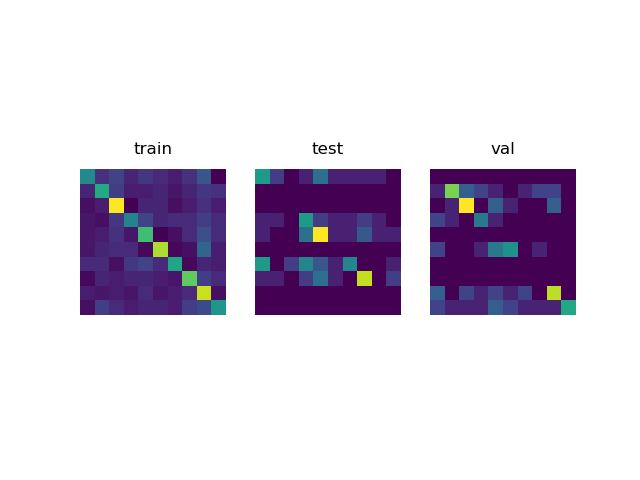
\includegraphics[width=0.7\linewidth]{img/confM}
	\caption{Матрицы неточностей для различных выборок.}
	\label{fig:confm}
\end{figure}


\subsection{Эксперимент с альбомом} 

Мы сравниваем эту модель с моделью и базовый уровень, который просто усредняет прогнозы single-imagePlaNet всех изображений в альбоме и назначает
среднее для всех изображений. Усреднение в альбомах ($ \mathcal{G}= \mathbb{E}[ \mathcal{F}(X) ] $) уже
дают значительное улучшение по сравнению с одним изображением PlaNet
(45,7\% на уровне улиц), поскольку у него больше
вмятины предсказания к неоднозначным изображениям. Однако, LSTM
модель явно превосходит технику усреднения (50,5\%
относительное улучшение уровня улицы). Визуальный контроль
результатов показали, что за достоверностью следуют несколько изображений с более низким местоположением уверенность, модель LSTM присваивает низкий уровень доверия изображения, расположенные вблизи изображения с высокой степенью достоверности в то время как $ \mathcal{F} $ может «прыгать» (менять предположение о расположении альбома), модель LSTM имеет тенденцию прогнозировать близкие местоположения, кроме случаев когда есть убедительные доказательства изменения местоположения. LSTM модель работает лучше усреднения из-за того что оно присваивает всем изображениям в альбоме одинаковые уровни значимости и не может производить точные прогнозы для альбомов которые включают разные местоположения (например, альбомы поездок).


\section{Результаты тестирования и примеры работы системы}

Нужно помнить, что пользователем может быть не только <<менеджер>> или <<человек в белом халате>>, но и другой программист. Последнее относится, в первую очередь, к реализованным библиотекам. Для <<обычных>> приложений нередко бывают пользователи нескольких категорий --- например, обычный пользователь и администратор. Для каждой категории нужно описать, как выполняются основные функции, предпочтительно, с помощью серии скрин-шотов. Однако считается плохим тоном вставлять длинную вереницу из скрин-шотов: если их много, большую часть нужно выносить в приложение. Для \textit{этого} раздела нормальной является плотность скрин-шотов из расчета: 1 страница скрин-шотов на 1-2 страницы текста.

\textit{\textbf{Замечание.}} В ПЗ (как УИРа, так и ВКР) следует избегать ситуаций, когда значительную часть основного содержания составляют страницы с иллюстрациями и таблицами, особенно, если такие страницы следуют подряд. В основном тексте следует оставлять лишь самые основные таблицы и рисунки, а остальное --- выносить в приложение.


\section{Сравнение реализованного программного обеспечения с существующими аналогами}

В сравнении должно быть отражено, чем полученное ПО выгодно (и невыгодно) отличается от прочих ближайших аналогов. Практика показывает, что аналоги есть всегда. А если нет аналогов, значит есть частичные решения, которые реализуют какие-то части функционала вашей системы. Тут тоже может быть относительно много таблиц и графиков.



\section{Выводы}

Следует перечислить, какие практические результаты были получены, а именно: какое программное или иное обеспечение было создано. В число результатов могут входить, например, методики тестирования, тестовые примеры (для проверки корректности/оценки характеристик тех или иных алгоритмов) и др. По каждому результату следует сделать вывод, насколько он отличается от известных промышленных аналогов и исследовательских прототипов.

